\section{Music Theory Applications}
\label{sec:music-theory-apps}
In order to establish what kinds of applications might exist in and around this music recognition and correction field, I researched online. The Apple ``App Store'' revealed several examples of applications which teach music theory, however none of these focus on writing music and are more based around ideas like flashcards and memorisation.

\begin{figure}[h!]
  \centering
  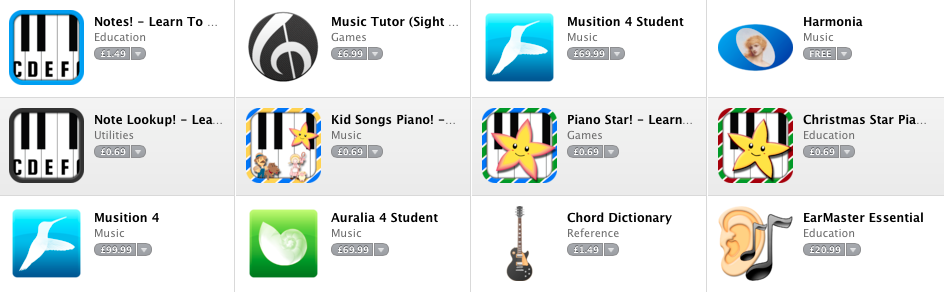
\includegraphics[width=\linewidth]{gfx/music-theory-apps.png}
  \caption{Music Theory Applications after searching ``Music Theory'' on the Apple App Store}
\end{figure}

Most of these apps however, are aimed at more advanced students and miss out a huge part of theory exams which is the written notation section.

\todo[inline,color=red]{Music Theory Apps - Add the other specific theory learning apps I looked at}
